\section{Durchführung}
\label{sec:Durchführung}

\subsection{Materialien und Versuchsaufbau}
Bei diesem Experiment soll das magnetische (Dipol-)Moment eines Permanentmagneten unter Ausnutzung zweier Verfahren bestimmt werden.
Der Permanentmagnet befindet sich dabei in einer Billiardkugel der Masse $m_{\text{K}}$. Das Dipolmoment $\mu_{\text{Dipol}}$ des Mageneten ist entlang eines Stiels,
welcher sich an der Kugel befindet, ausgerichtet. In diesen Stiel lässt sich wiederum eine kleine Aluminiumstange befestigen, an der eine Masse $m$ verschoben werden kann.


Die Billiardkugel wird für beide Verfahren in ein homogenes Magnetfeld gesetzt. Dies geschieht mit Hilfe eines Helmholtz-Spulenpaares, in dessen Mitte sich eine
Messinghalterung befindet, auf der die Kugel abgelegt werden kann. In der Halterung befinet sich ein Loch, über das ein \glqq Luftkissen\grqq \: erzeugt werden kann, auf dem
die Kugel reibungsarm gelagert ist. Die Apparatur wird über ein Steuergerät reguliert. An diesem lässt sich das Luftkissen einschalten, die Feldrichtung
des Magnetfeldes anpassen und die Stromstärke einstellen. Die Stromstärke kann an einer analogen Anzeige abgelesen werden. Der Aufbau kann \autoref{fig:Aufbau} entnommen werden.

\begin{figure}
    \centering
    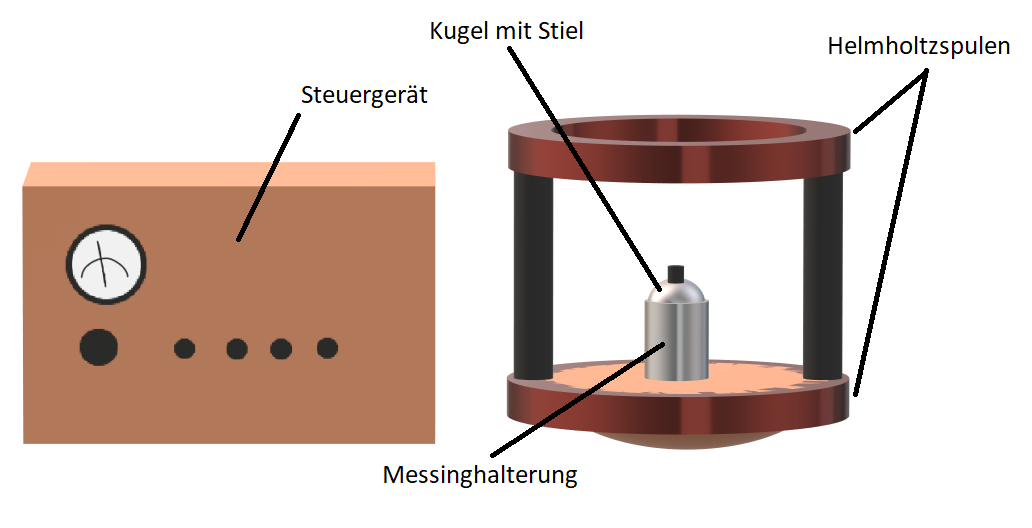
\includegraphics[width=\textwidth]{content/AufbauSkizze.png}
	\caption{Skizze des Versuchaufbaus. \cite{paint3d}}
	\label{fig:Aufbau}
\end{figure}

Vor der eigentlichen Durchführung der Messung müssen alle Apparatenkonstanten festgestellt werden. Dazu zählen die Eigenschaften des Helmholtzspulenpaares, die Massen der 
Kugel und der beweglichen Masse, sowie die geometrischen Abmessungen der Kugel. Die Werte für die Maße der Kugel und die Massen finden sich in \autoref{sec:Auswertung}.
Das Helmholtzspulenpaar hat $N = 195$ Windungen, die einzelnen Spulen einen Radius von $R_{\text{Spule}} = 0.109\unit{\metre}$ und der Abstand der Spulen beträgt
$d = 0.138\unit{\meter}$.

\subsection{Vorbereitungsaufgaben}
\label{subsec:Vorbereitungsaufgaben}

Zur Vorbereitung sollte der Betrag der Flussdichte $B$ in der Mitte des Spulenpaares bei einem Strom von $I = 1\unit{\ampere}$ und das Trägheitsmoment $J_{\text{K}}$
einer Kugel mit Radius $r_k = 2.5\unit{\centi\metre}$ und Masse $m_k = 150\unit{\gram}$ bestimmt werden.
Ersteres berechnet sich nach \autoref{eqn:Helmholtz_B} zu:
\begin{equation*}
    B = 195 \cdot \frac{\mu_0 1\unit{\ampere}(0.109\unit{\metre})^2}{((0.109\unit{\metre})^2 + (0.5 \cdot 0.138\unit{\meter})^2)^{3/2}} = 1.356 \unit{\milli\tesla}
\end{equation*}
(Magnetische Feldkonstante $\mu_0 = 1.25663706212 \cdot 10^{-6} \unit{\newton\per\ampere\squared}$ \cite{scipy}) \\
Das Trägheitsmoment ergibt sich nach \autoref{eqn:Trägheitsmoment_Kugel} zu:
\begin{equation*}
    J_{\text{K}} = \frac{2}{5} \cdot 0.150\unit{\kilogram} \cdot (0.025\unit{\metre})^2 = 3.75 \cdot 10^{-5} \unit{\kilogram\metre\squared} 
\end{equation*}

\subsection{Methode 1: Ausnutzung der Erdgravitation}
\label{subsec:Methode1}

Bei der ersten Methode zur Bestimmung des Dipolmoments wird ein Kräftegleichgewicht zwischen der Gravitationskraft $F_g$ und der magnetischen Kraft, die auf den Dipol 
wirkt, ausgenutzt. Dazu wird der Aluminiumstab in die Kugel gesteckt. Auf diesem kann nun eine kleine Masse vertikal verschoben werden. Die Kugel wird in der Messinghalterung platziert
und das Luftkissen eingeschaltet. Die Magnetfeldrichtung muss dabei auf \dq up\dq \: eingestellt sein. Solange kein Strom fließt gibt es kein Magnetfeld, was zur Folge hat,
dass der Aluminiumstab auf dem Gestell der Helmholtzspulen aufliegt. Wird nun der Strom eingeschaltet wirkt das Magnetfeld der Gravitationskraft entgegen.
Auf den Dipol wirken nun zwei Drehmomente: eines auf Grund des Magnetfeldes, da Dipole sich parallel zu diesem ausrichten wollen, und eines, welches an der 
verschiebbaren Masse angreift und durch die Wirkung der Gravitation auf diese Masse verursacht wird. \\
Wird nun die Stromstärke langsam erhöht stellt sich an einem gewissen Punkt ein Gleichgewicht ein, bei dem die Kugel samt Stab in einer stabilen Position verweilt.
Dabei ist darauf zu achten, dass die Kugel nicht rotiert, da es sonst zu Präzessionseffekten kommen kann. \\
Mit diesem Verfahren wird nun bei verschiedenen Abständen $r$ der verschiebbaren Masse zur Kugel der Gleichgewichtszustand eingestellt und die Stromstärke $I$ zu jedem $r$ notiert. 
Dies wird für mindestens neun Wertepaare wiederholt.

\subsection{Methode 2: Bestimmung des magnetischen Moments über die Schwingungsdauer}
\label{subsec:Methode2}

Bei der zweiten Methode befindet sich die Kugel im Magnetfeld auf dem Luftkissen. Der Aluminiumstab ist nicht montiert. Wird nun die Kugel um einen \textbf{kleinen Winkel}
aus der Ruhelage (Stiel oben) ausgelenkt, wirkt -- wie bei der ersten Methode -- ein Drehmoment auf den Dipol. Dieses Drehmoment wirkt als rückstellende Kraft,
sodass die Billiardkugel wieder in Richtung der Ruhelage beschleunigt wird. Die Kugel führt nun eine Schwingung aus, da sie immer wieder über die Ruhelage hinaus schwingt.
Die ausgeführte Schwingung ist die eines harmonischen Oszillators mit Schwingungsdauer $T$. \\
Zur Messung wird nun die Stromstärke $I$ variiert und die Kugel mit Hilfe des Stiels aus der Ruhelage ausgelenkt. Es werden 10 Schwingungsdauern abgezählt und die Zeit ($10 \,T$) 
mit einer Stoppuhr gemessen. Beide Werte werden notiert und das Messverfahren wird für mindestens 9 andere Stromstärken wiederholt.
Das Messen von 10 Schwingungsdauern hat den Grund, dass grade bei großen Stromstärken eine einzelne Schwingungsperiode sehr kurz ist und somit eine Ungenauigkeit beim Stoppen
mit der Stoppuhr zu großen Abweichungen führen kann. Zusätzlich wurde in unserem Fall die Zeit auf zwei verschiedenen Stoppuhren unabhängig voneinander gestoppt, um den 
Messumfang zu erhöhen und eventuelle Ungenauigkeiten, die durch den Experimentator verursacht werden könnten, heraus mitteln zu können.
Die beiden 10 fachen Periodendauern werden anschließend zu einem Wert für eine Schwingungsdauer $T$ gemittelt.
 